\documentclass[12pt]{article}
\usepackage{amsfonts,amsmath,amssymb,graphicx,url,tikz,amsthm}
\usetikzlibrary{arrows,automata}

% Old Stuff
%%\oddsidemargin=0.15in
%%\evensidemargin=0.15in
%%\topmargin=-.5in
%%\textheight=9in
%%\textwidth=6.25in

\setlength{\oddsidemargin}{.25in}
\setlength{\evensidemargin}{.25in}
\setlength{\textwidth}{6.25in}
\setlength{\topmargin}{-0.4in}
\setlength{\textheight}{8.5in}

\newcommand{\heading}[5]{
   \renewcommand{\thepage}{#1-\arabic{page}}
   \noindent
   \begin{center}
   \framebox{
      \vbox{
    \hbox to 6.2in { {\bf MS205 Automata Theory}
     	 \hfill #2 }
       \vspace{4mm}
       \hbox to 6.2in { {\Large \hfill #5  \hfill} }
       \vspace{2mm}
       \hbox to 6.2in { {\it #3 \hfill #4} }
      }
   }
   \end{center}
   \vspace*{4mm}
}

\newcommand{\handout}[3]{\heading{#1}{#2}{Huang Zen 5120309027}{}{#3}}

\setlength{\parindent}{0in}
\setlength{\parskip}{0.1in}

\begin{document}
\handout{1}{Dec 12, 2013}{Problem Set 1}

\paragraph{Problem 1} 
\begin{itemize}
\item[1.]
\begin{tikzpicture}[->,>=stealth',shorten >=1pt,auto,node distance=2.8cm,
                    semithick]
	\node[state,initial]		(0)				{$q_0$};
	\node[state]			(1)	[right of = 0]	{$q_1$};
	\node[state,accepting]	(2) 	[right of = 1]	{$q_2$};
	\path[->] 	(0)	edge[loop above]	node{1}	()
				edge	[bend left]		node{0}	(1)
			(1)	edge[loop above]	node{1}	()
				edge	[bend left]		node{0}	(2)
			(2)	edge[loop above]	node{1}	()
				edge	[bend left]		node{0}	(0);
\end{tikzpicture}	
\item[2.]
\begin{tikzpicture}[->,>=stealth',shorten >=1pt,auto,node distance=2.8cm,
                    semithick]
	\node[state,initial,accepting]		(00)					{$q_{00}$};
	\node[state]					(01)	[right of = 00]		{$q_{01}$};
	\node[state]					(02) 	[right of = 01]		{$q_{02}$};
	\node[state]					(10)	[below of = 00]		{$q_{10}$};
	\node[state]					(11)	[right of = 10]		{$q_{11}$};
	\node[state]					(12) 	[right of = 11]		{$q_{12}$};
	\path[->] 	(00)	edge	[bend right]			node{0}	(10)
				edge	[bend right]			node{1}	(01)
			(01)	edge	[bend right]			node{0}	(11)
				edge	[bend right]			node{1}	(02)
			(02)	edge	[bend right]			node{0}	(12)
				edge	[bend right]			node{1}	(00)
			(10)	edge	[bend right]			node{0}	(00)
				edge	[bend left]				node{1}	(11)
			(11)	edge	[bend right]			node{0}	(01)
				edge	[bend left]				node{1}	(12)
			(12)	edge	[bend right]			node{0}	(02)
				edge	[bend left]				node{1}	(10);
\end{tikzpicture}	
\item[3.]
Since the problem isn't clear enough,
take it as searching for 6 consecutive $0$s.

\begin{tikzpicture}[->,>=stealth',shorten >=1pt,auto,node distance=2cm,
                    semithick]
	\node[state,initial]				(0)					{$q_{0}$};
	\node[state]					(1)	[right of = 0]		{$q_{1}$};
	\node[state]					(2) 	[right of = 1]		{$q_{2}$};
	\node[state]					(3)	[right of = 2]		{$q_{3}$};
	\node[state]					(4)	[right of = 3]		{$q_{4}$};
	\node[state]					(5) 	[right of = 4]		{$q_{5}$};
	\node[state,accepting]			(6) 	[right of = 5]		{$q_{6}$};
	\path[->] 	(0)	edge	[loop above]				node{1}	()
				edge	[bend right]			node{0}	(1)
			(1)	edge[bend left]				node{1}	(0)
				edge[bend right]			node{0}	(2)
			(2)	edge[bend left]				node{1}	(0)
				edge[bend right]			node{0}	(3)
			(3)	edge[bend left]				node{1}	(0)
				edge[bend right]			node{0}	(4)
			(4)	edge[bend left]				node{1}	(0)
				edge[bend right]			node{0}	(5)
			(5)	edge[bend left]				node{1}	(0)
				edge[bend right]			node{0}	(6)
			(6)	edge[loop above]				node{0,1}	();

\end{tikzpicture}	
\end{itemize}

\bigskip

\paragraph{Problem 2} 
\begin{proof}
We show it by contradiction.

Suppose that the number of subsets  of the set of all finite length strings,
which is equivalent to the number of functions from elements to $\{0, 1\}$ is countably infinite,
so that we can label these functions $\{f_1, f_2, ..., f_n, ...\}$ with distinct integers of $\mathbb{N}$.
We can also label all finite length strings $\{s_1, s_2, ..., s_n, ...\}$,
such like first by length and second by dictionary order,
since we already know their number is countably infinite.
Given one such labeling, we form a function $f_p$ as following:
$$
f_p(s_i) \not= f_i(s_i)
$$
saying equivalently we construct a subset containing the $i$th string while the $i$th subset not,
or to the contrary.
We can easily see $f_p$ is not in any $f_i$ since it differs from any $f_i$ at $s_i$,
this is contradict to our assumption.
So the number of subsets of the set of all finite length strings is not countably infinite.
\end{proof}
\bigskip

\paragraph{Problem 3} 
\begin{itemize}
\item[1.]
Countably infinite.
Number of strings of every fixed length is finite.
And we can order strings first by length second by dictionary order.
\item[2.]
Countably infinite.
Clearly it's at least countably infinite,
and any finite automata can be expressed by certain string of finite length.
\item[3.]
Countably infinite.
The reason is the same as for finite automata.
\item[4.]
Not countably infinite.
The proof is similar to Problem 2.
\item[5.]
Not countably infinite.
The proof is similar to Problem 2.

\end{itemize}
\end{document}








